\documentclass[a4paper,11pt]{refart}

\usepackage[utf8]{inputenc}
\usepackage[T1]{fontenc} % LY1 also works

%% Font settings suggested by fbb documentation.
\usepackage{textcomp} % to get the right copyright, etc.
\usepackage[lining,tabular]{fbb} % so math uses tabular lining figures
\usepackage[scaled=.95,type1]{cabin} % sans serif in style of Gill Sans
\usepackage[varqu,varl]{zi4}% inconsolata typewriter
\useosf % change normal text to use proportional oldstyle figures
%\usetosf would provide tabular oldstyle figures in text

\usepackage{microtype}

\usepackage{graphicx}
\usepackage{enumitem}
\setlist{leftmargin=*}
\usepackage{listings}
\lstset{basicstyle=\ttfamily,frame=single,xleftmargin=3em,xrightmargin=3em}
\usepackage[os=win]{menukeys}
\renewmenumacro{\keys}[+]{shadowedroundedkeys}
\usepackage{framed}
\usepackage{etoolbox}
\AtBeginEnvironment{leftbar}{\sffamily\small}

\usetikzlibrary{chains,arrows,shapes,positioning}
\usepackage{hyperref}

\usepackage{fontawesome5}
\usepackage{float}

\newcommand\AutoCalc{\textsf{AutoratingCalculator}}
\newcommand\Ranqhana{\textsf{Ranqhana}}
\newcommand\SiteRanqhana{\textsf{http://localhost:4200/}}
\renewcommand\abstractname{Introduction}

\title{Ranqhana User Guide}
\author{Jose Clavo Tafur (\url{jclavotafur@gmail.com})}
%	\\\url{http://liantze.penguinattack.org}}
\date{\url{https://ai-apaec.com/product/ranqhana}\\May, 2021}
\begin{document}
\maketitle

\begin{abstract}
 \Ranqhana{} is a manager software for your store (restaurant, supermarket, shop and others), it has the next modules: dashboard, invoices, orders, products, services, persons and reports. Where it is possible to purchase and sell items, in addition to manage products and services as well some reports. Available for rent at \url{https://ai-apaec.com/product/ranqhana}. It will be needed only a connection to internet and a browser to access and use the system.
\end{abstract}

\tableofcontents
\clearpage

\section*{Quick Guide to Workflow}

%\begin{enumerate}
%\item 
%\end{enumerate}

%\begin{tikzpicture}
%\tikzset{every node/.style={on chain,draw,thick,rounded corners,
%minimum height=3em, text width=10em, align=center}}
%\begin{scope}[start chain=going below]
%\node (prepare-group) {Prepare group list (\texttt{.csv})};
%\node (import-group) {Import group list for new score file (\texttt{.xml})};
%\node (enter-rating) {Enter peer ratings given by each student};
%\node (compute-score) {Compute autorated weights and scores};
%\node (export-csv) {Export data for Excel (\texttt{.csv})};
%\end{scope}
%\node[right=of enter-rating] (open-score) {Open previously saved score file (\texttt{.xml})};
%
%\path[draw,line width=0.4ex, ->,>= angle 60]
%(prepare-group) edge (import-group) 
%(import-group) edge (enter-rating)
%(open-score) edge (enter-rating)
%(enter-rating) edge (compute-score) 
%(compute-score) edge (export-csv);
%\end{tikzpicture}


\section{Login Module}

\subsection{Login in the application}
\begin{enumerate}
\item Go to \SiteRanqhana
\item Write your identification, \emph{which is in a numeric format}
\item Write your password
\item Click in \keys{login}
\begin{figure}[H]\centering
	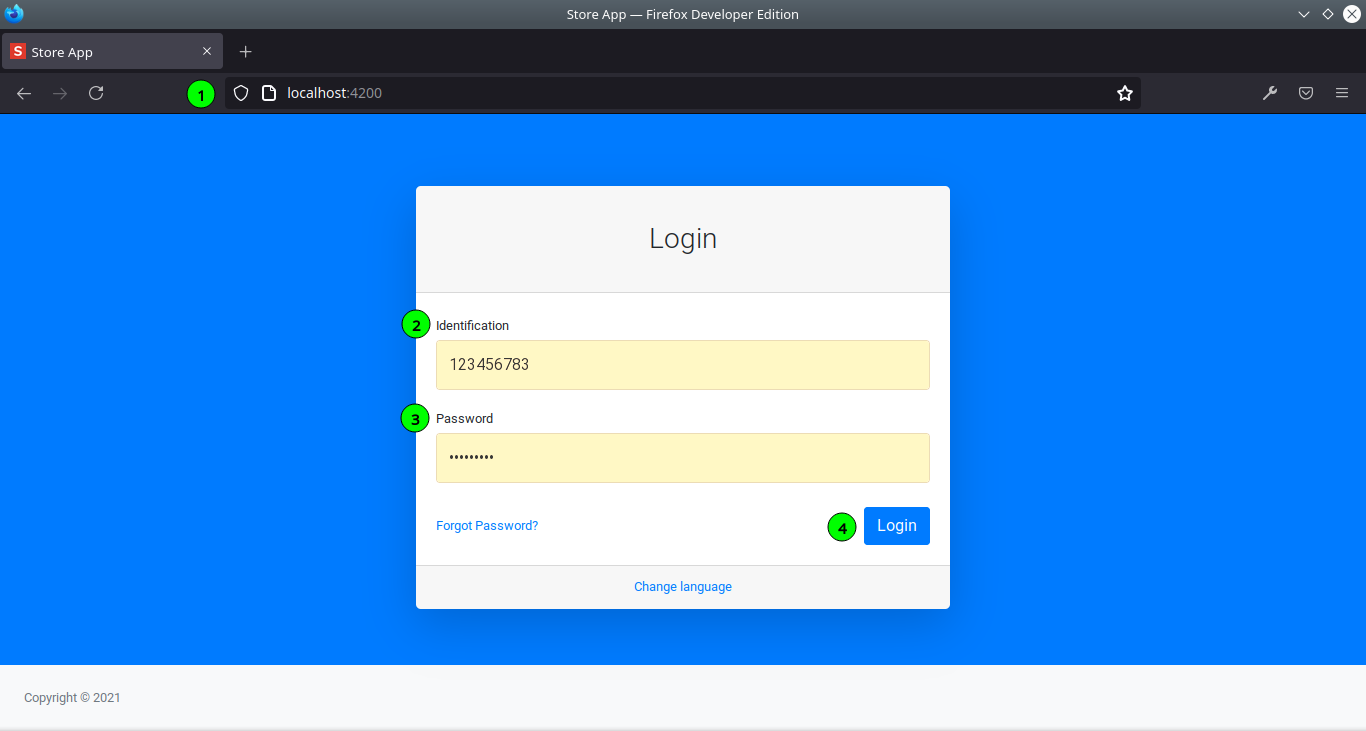
\includegraphics[width=\textwidth]{images/login}
	\caption{Login in the application}\label{fig:login}
\end{figure}
\end{enumerate}	


\subsection{Change language}
\begin{enumerate}
	\item Click in ...
\end{enumerate}	

\section{Invoices Module}

\subsection{To Sell}
\subsubsection{Access to the module}
\begin{enumerate}
	\item From the left menu, click in  \menu{Invoices}
	\item From the left submenu, click in  \menu{Sell invoice}
	\item The page will be showed.
	\begin{figure}[H]\centering
		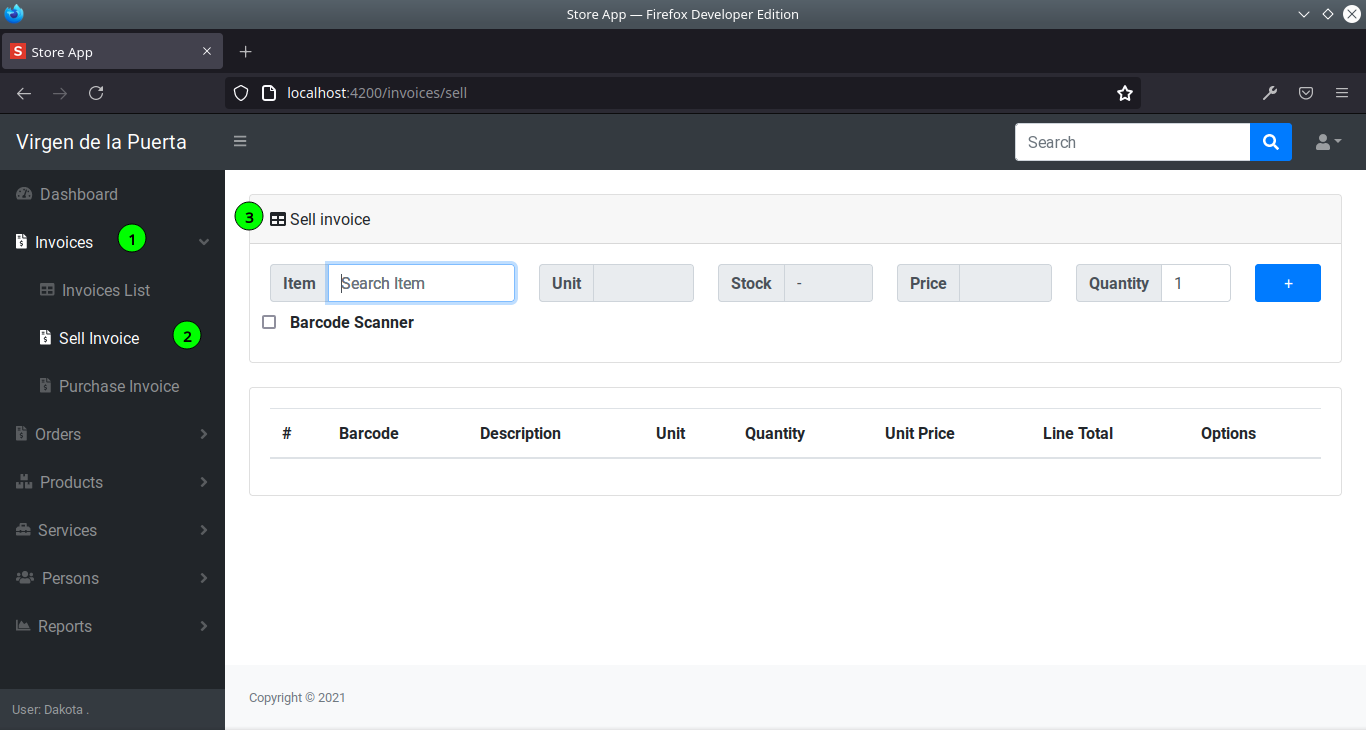
\includegraphics[width=\textwidth]{images/sellinvoice-1}
		\caption{Access to the module}\label{fig:sellinvoice-1}
	\end{figure}
\end{enumerate}

\subsubsection{Add an item}
\begin{enumerate}
	\item Search item, \emph{write the first letters of item name and it will be auto-completed.}
	
	\medskip
	\begin{leftbar}
		It will show item's information such as \emph{ unit, stock and price}
	\end{leftbar}
	\item Write quantity.
	\item Click in \keys{\texttt{+}}
	\item The item will be showed in the grill,  \emph{with some additional information}
	\begin{figure}[H]\centering
		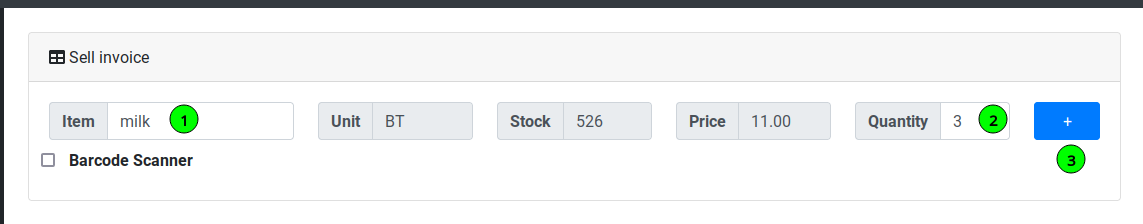
\includegraphics[width=\textwidth]{images/sellinvoice-2}
		\caption{Add an item}\label{fig:sellinvoice-2}
	\end{figure}
\end{enumerate}

\subsubsection{Show item in the grill}
\begin{enumerate}
	\item in that section, the item is showed in the grill,  \emph{with some additional fields}
	\medskip
	\begin{leftbar}
		It will show item's information such as \emph{ index, barcode, unit, quantity, unit price, line total and delete button}
	\end{leftbar}
	\item in that section, information about \emph{subtotal, taxes, discount and total} is showed
	\medskip
	\begin{leftbar}
	To make a discount check its section
	\end{leftbar}
	\begin{figure}[H]\centering
		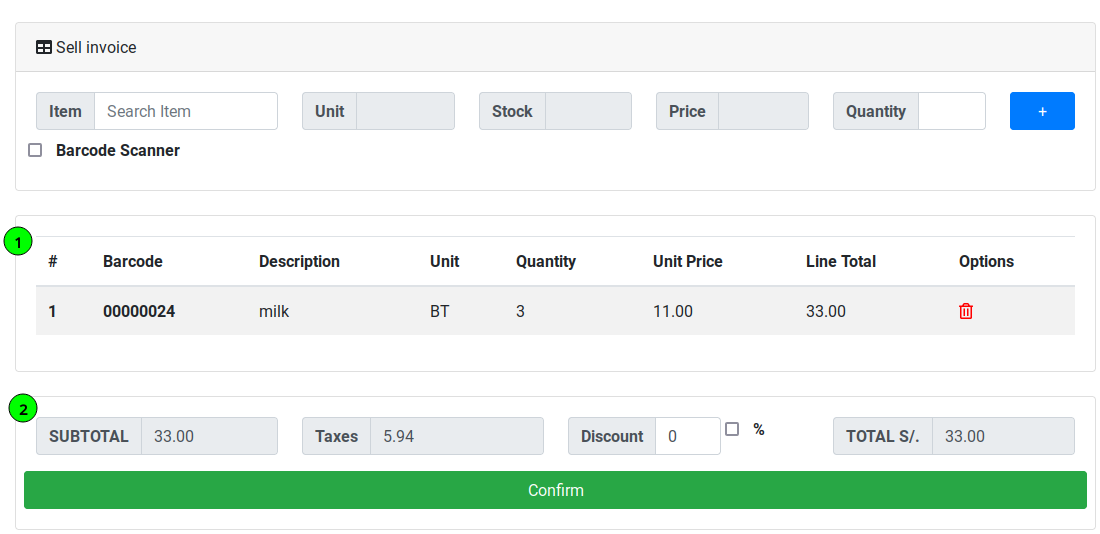
\includegraphics[width=\textwidth]{images/sellinvoice-3}
		\caption{Show item in the grill}\label{fig:sellinvoice-3}
	\end{figure}
\end{enumerate}

\subsubsection{confirm the sell}
\begin{enumerate}
	\item Click in \keys{Confirm} 
	\begin{figure}[H]\centering
		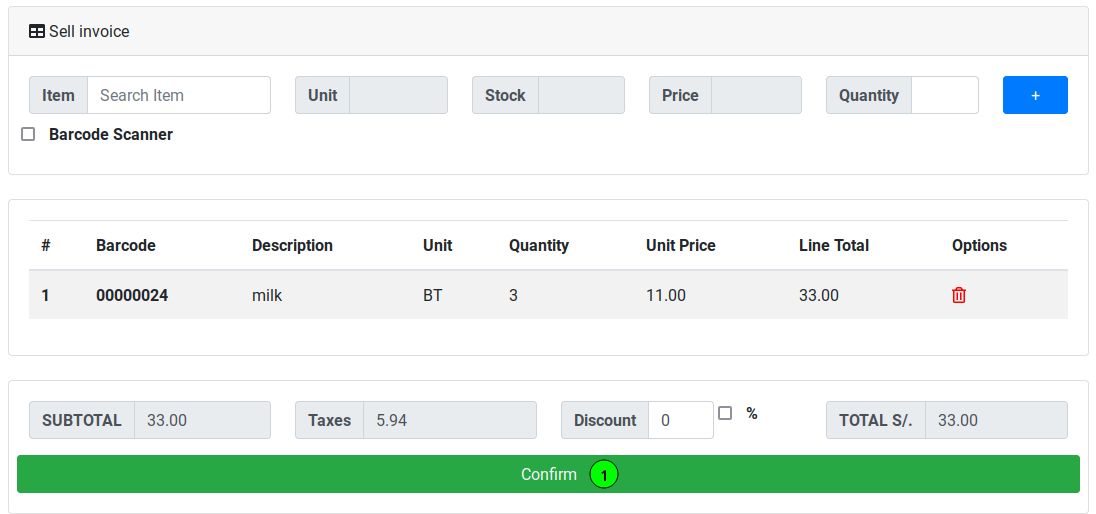
\includegraphics[width=\textwidth]{images/sellinvoice-4}
		\caption{confirm the sell}\label{fig:sellinvoice-4}
	\end{figure}
\end{enumerate}

\subsubsection{Add additional information}
about \emph{payment type} there are the next options:
\begin{itemize}
	\item Credit
	\item Debit
	\item Cash
	\item Store Credit
\end{itemize}

\subsubsection{Add additional information: Credit or Debit}
\begin{enumerate}
	\item Select payment type \textbf{CREDIT} or \textbf{DEBIT}	
	\item Select a client, \emph{write its name or identification number}
	\medskip
	\begin{leftbar}
		\textbf{OPTIONAL FIELD}
	\end{leftbar}
	\item Click in \keys{Finish} 	
	\medskip
	\begin{leftbar}
		the process will be finished and the user will redirected to \textbf{Invoice List} page.
	\end{leftbar}
	\begin{figure}[H]\centering
		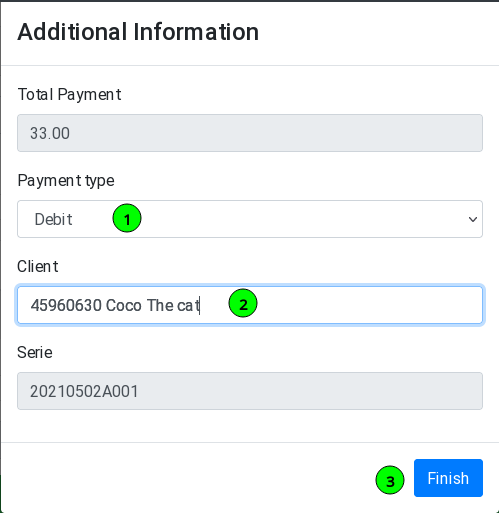
\includegraphics[width=\textwidth]{images/sellinvoice-5}
		\caption{Add additional information: Credit or Debit}\label{fig:sellinvoice-5}
	\end{figure}
\end{enumerate}

\subsubsection{Add additional information: Cash}
\begin{enumerate}
	\item Select payment type \textbf{CASH}	
	\item Select a client, \emph{write its name or identification number}
	\medskip
	\begin{leftbar}
		\textbf{OPTIONAL FIELD}
	\end{leftbar}
	\item Click in \keys{Next} 	
	\medskip
	\begin{figure}[H]\centering
		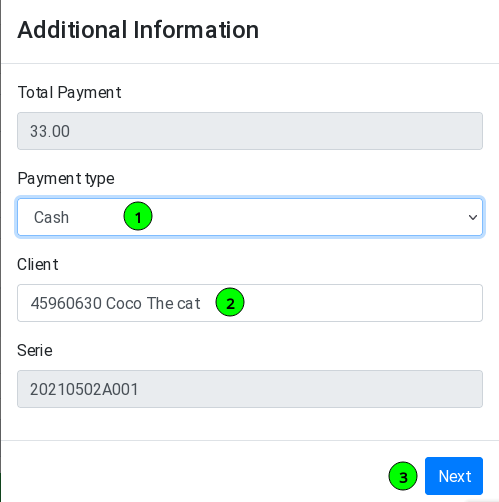
\includegraphics[width=\textwidth]{images/sellinvoice-6}
		\caption{Add additional information: Cash}\label{fig:sellinvoice-6}
	\end{figure}
\end{enumerate}

\subsubsection{Made Payment}
\begin{enumerate}
	\item Write the amount of cash 
	\item If there is an exchange, it will be showed
	\item Click in \keys{Pay}
	\medskip
	\begin{leftbar}
		the process will be finished and the user will redirected to \textbf{Invoice List} page.
	\end{leftbar}
	\begin{figure}[H]\centering
		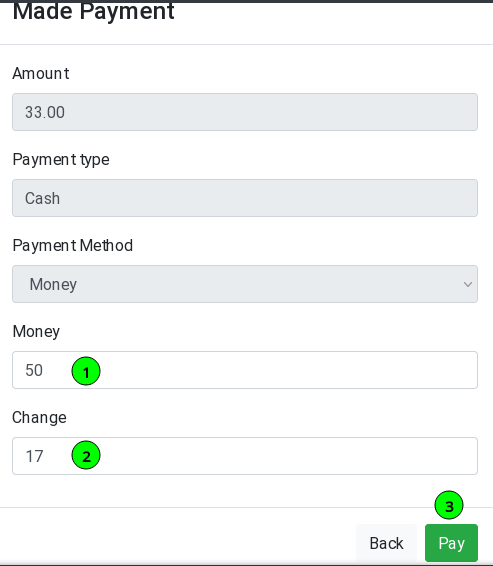
\includegraphics[width=\textwidth]{images/sellinvoice-7}
		\caption{Made Payment}\label{fig:sellinvoice-7}
	\end{figure}
\end{enumerate}

\subsubsection{Show sell invoice}

\section{Product}

\subsection{Product List}

\subsubsection{Access to the module}
\begin{enumerate}
	\item From the left menu, click in  \menu{Products}
	\item From the left submenu, click in  \menu{Products List}
	\item The page will be showed.
	\medskip
	\begin{leftbar}
		Here there are some action that can be done with the items in the grid such as:  \emph{search, edit, delete and print} .
	\end{leftbar}
	\begin{figure}[H]\centering
		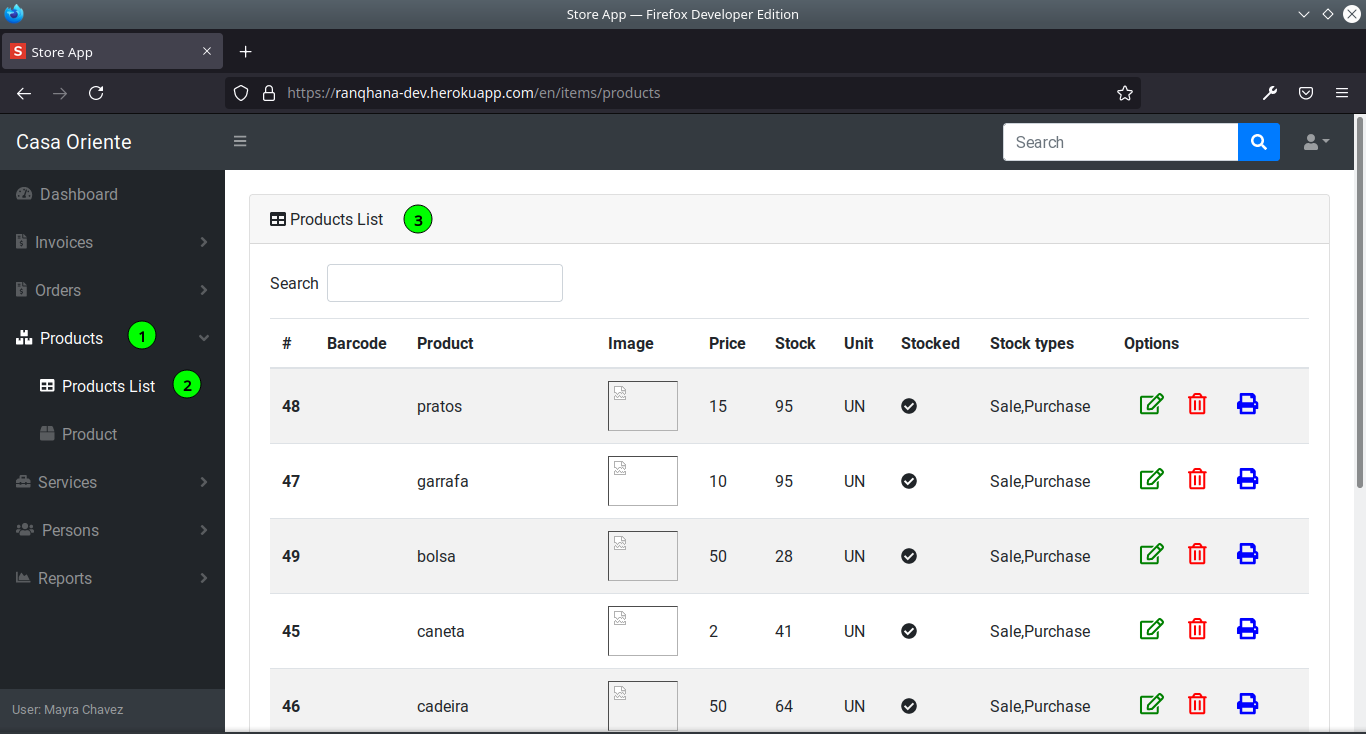
\includegraphics[width=\textwidth]{images/produc_list-access.png}
		\caption{Access to the module: Product List}
		\label{fig:produc_list-access.png}
	\end{figure}
\end{enumerate}

\subsubsection{Search product}
\begin{enumerate}
	\item Write the product name or part of that and it will be searched automatically.
	\begin{figure}[H]\centering
		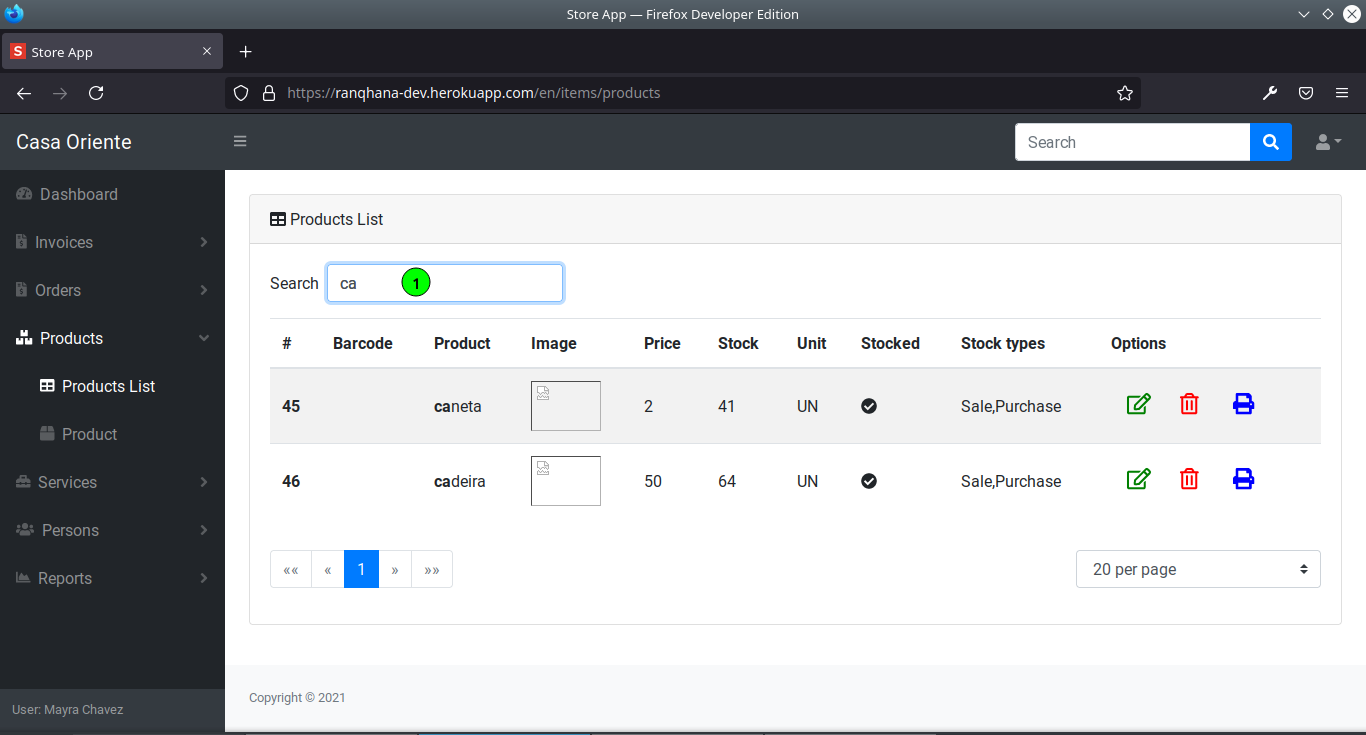
\includegraphics[width=\textwidth]{images/produc_list-search.png}
		\caption{search product}
		\label{fig:produc_list-search.png}
	\end{figure}
\end{enumerate}

\subsubsection{Delete product}
\begin{enumerate}
	\item Find the product to delete.
	\item Click in \faIcon{trash}.
		\begin{figure}[H]\centering
			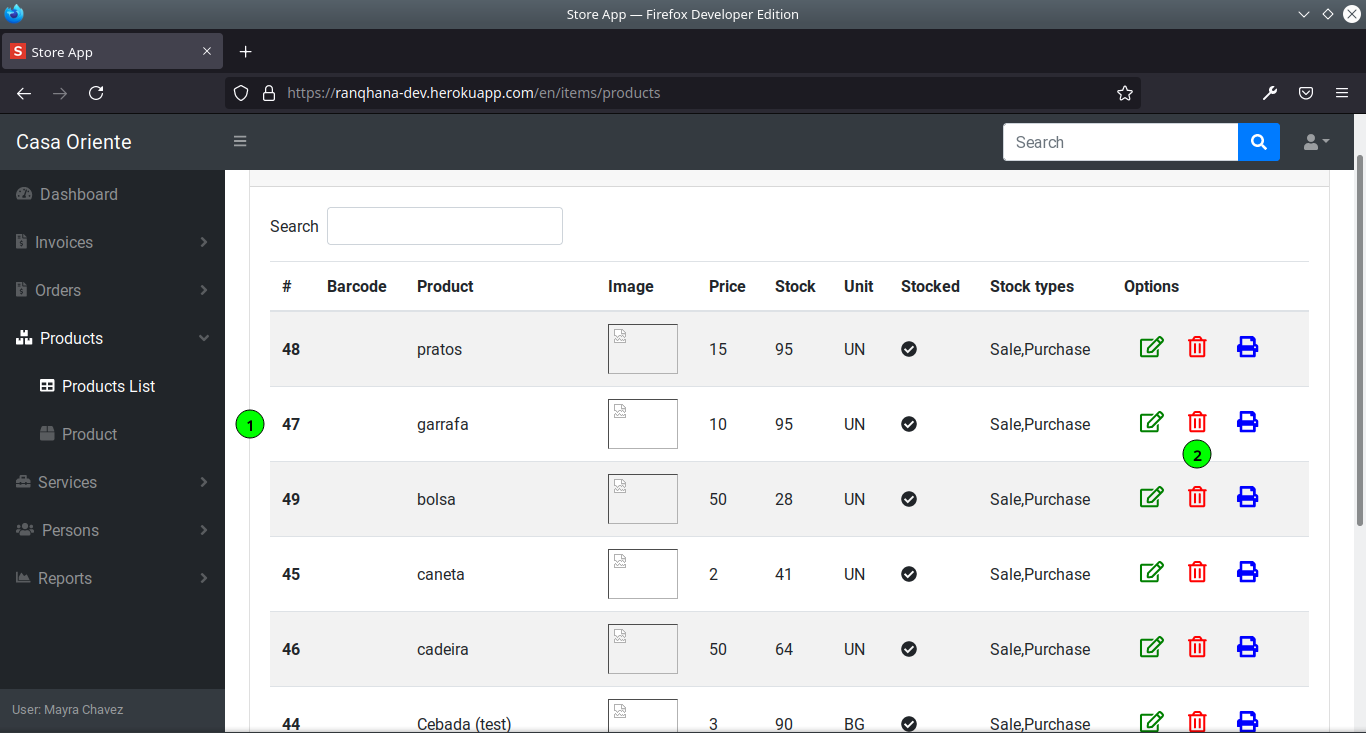
\includegraphics[width=\textwidth]{images/produc_list-delete.png}
			\caption{delete product}
			\label{fig:produc_list-delete.png}
		\end{figure}
	\item Click in \keys{yes} to confirm the delete; otherwise, Click in \keys{cancel} to abort the process.
	\begin{figure}[H]\centering
		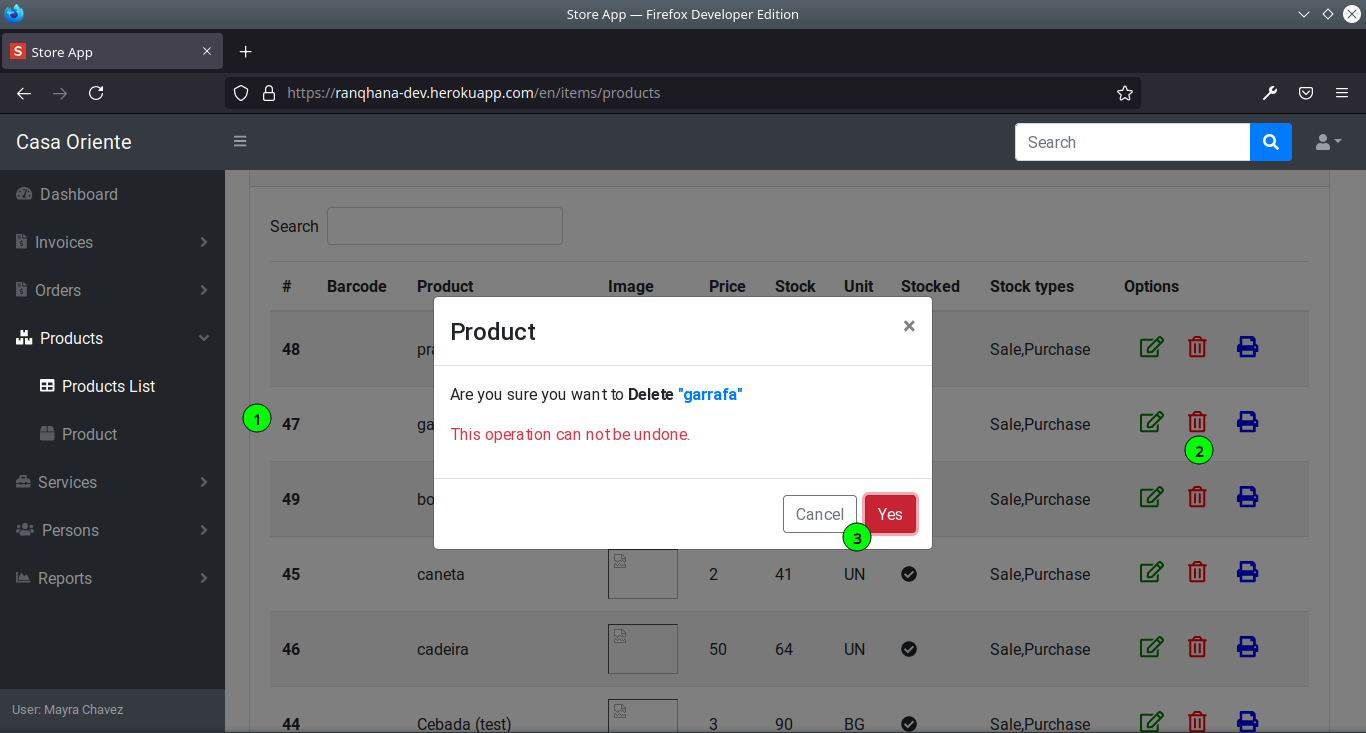
\includegraphics[width=\textwidth]{images/produc_list-delete-popup.png}
		\caption{delete product: popup}
		\label{fig:produc_list-delete-popup.png}
	\end{figure}
\end{enumerate}

\subsubsection{Update/Edit product}
\begin{enumerate}
	\item Find the product to edit.
	\item Click in \faIcon{edit}.
	\begin{figure}[H]\centering
		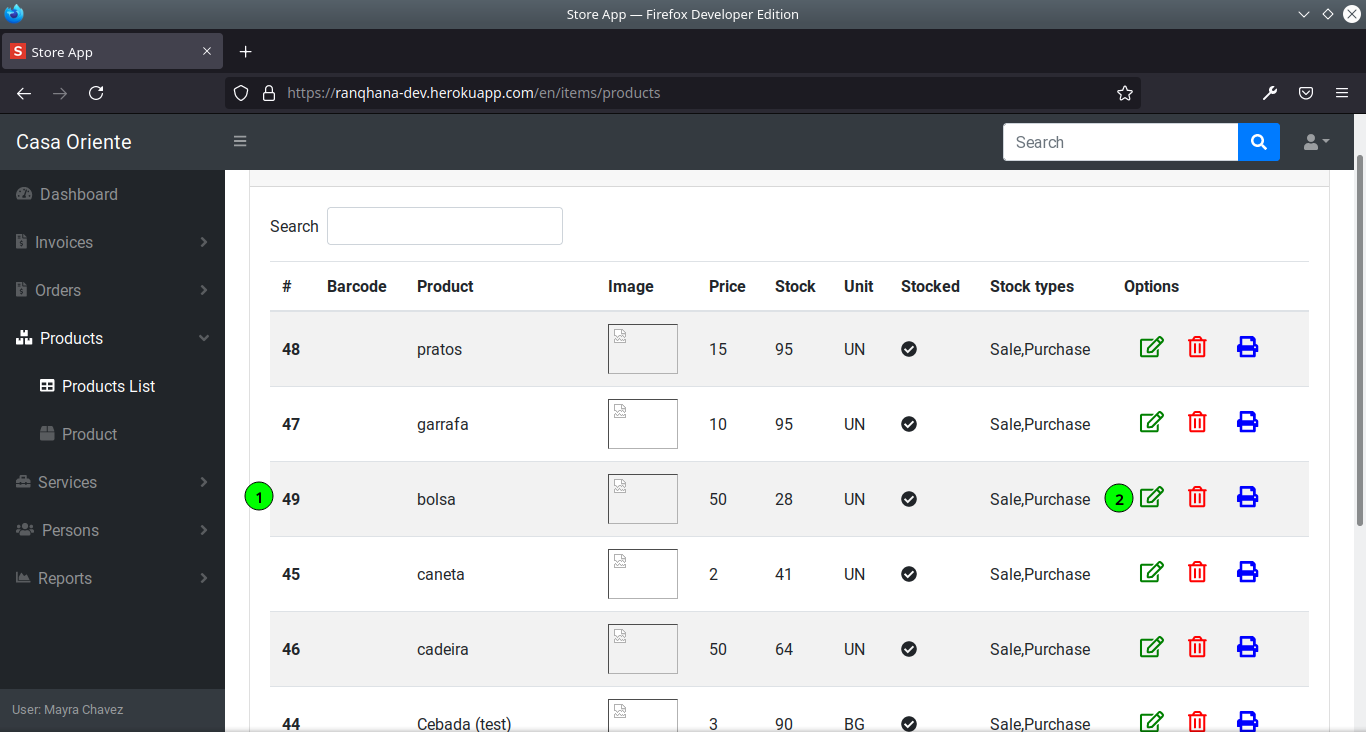
\includegraphics[width=\textwidth]{images/produc_list-update.png}
		\caption{update/edit product}
		\label{fig:produc_list-update.png}
	\end{figure}
\end{enumerate}

\subsection{Product Form}

%\begin{enumerate}
%	
%\begin{lstlisting}
%10032,Mary Tan
%10143,Prabakar Murugan
%10033,Tan Beng Huat
%10165,Calvin Ong
%
%10052,Mooi Siok Lan
%10114,Bong Chin Keat
%10432,Joseph Calvin
%10281,Suresh Kappan
%\end{lstlisting}
%  
%\item Save the group list file using \texttt{.txt} or \texttt{.csv} extension, e.g.\\\texttt{DIT1234-Apr2013-groups.txt}.
%
%\medskip
%
%\begin{leftbar}
%You may also prepare the group list in Excel. List the IDs in column A and the IDs in column B. Save the file as a Comma separated values file (CSV). In the Export Filter Settings, set text delimiter to blank, and field separator to comma (\texttt{,}).
%\end{leftbar}
%
%\end{enumerate}
%
%\section{Importing a Group List for a New Assignment Score File}
%
%\begin{enumerate}
%\item Launch the \AutoCalc\ tool by double-clicking on its icon in Windows Explorer.
%\item From the menu bar, select \menu{File>Import...} or press \keys{Ctrl+I}.
%\item Select a \emph{group list file} (\texttt{*.txt, *.csv}) to import from, e.g.\\\texttt{DIT1234-Apr2013-groups.txt}.
%\item \AutoCalc\ will then ask you for a \emph{new} file name to save the new score list as (\texttt{*.xml}), e.g.~\texttt{DIT1234-Apr2013-Assgn1.xml}.
%
%
%\medskip
%
%\begin{leftbar}
%Make sure the \texttt{.xml} score filename selected does not already exist. Otherwise the existing score file \textbf{may be overwritten without warning}!
%\end{leftbar}
%
%\medskip
%
%\item \AutoCalc\ imports the group lists and displays the student IDs and names in the main panel (Figure~\ref{fig:grouplist}).
%
%\begin{figure}[H]\centering
%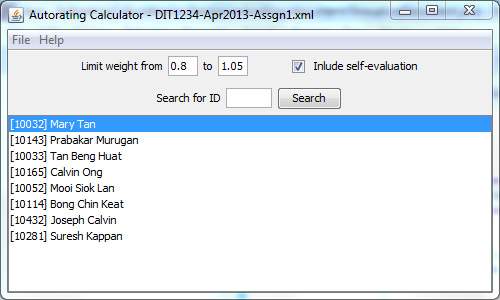
\includegraphics[width=\textwidth]{images/grouplist}
%\caption{Imported group list}\label{fig:grouplist}
%\end{figure}
%\end{enumerate}
%
%\section{Computing Autorated Scores from Group Scores and Peer Ratings}
%
%\subsection{Setting Options}
%
%Two options may be set at the top of the main \AutoCalc{} window.
%
%\begin{itemize}
%\item You may set the minimum and maximum autorating weight caps. Defaults are set at 0.8 and 1.02.
%
%\item You may choose whether to include self-evaluated peer ratings. The default is to include self ratings.
%
%\item If you change the settings, make sure to save them from the menu \menu{File>Save} or pressing \keys{Ctrl+S}.
%\end{itemize}
%
%\subsection{Selecting Students from List}
%
%Double-click on the name of a student in the list to display the peer review score entry window.
%
%\subsection{Searching Students by ID}
%
%You can also load the peer ratings entry window of a student by keying in the ID number in the search box, and then click on the \keys{Search} button.
%
%\subsection{Entering Scores and Ratings}
%
%\begin{enumerate}
%\begin{figure}[H]
%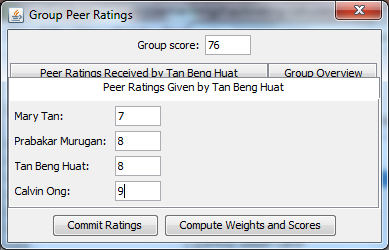
\includegraphics[width=\textwidth]{images/scorewindow}
%\caption{Peer Ratings Window}
%\end{figure}
%
%\item In the peer ratings window for each student, enter the peer ratings given by the student to his/her teammates, including him/herself.
%\item Enter also the overall score awarded to the group at the top of the window. (You only need to enter the group score once for each group.)
%\item Click the  \keys{Commit Ratings} button to save the ratings.
%\item Close the current peer rating window. Continue entering scores for other students.
%\item You may click on the \keys{Peer Ratings Received by \ldots} tab to see ratings received by a student.
%
%\begin{figure}[H]
%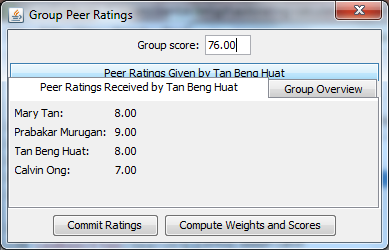
\includegraphics[width=\textwidth]{images/ratingsreceived}
%\caption{Peer Ratings Received}
%\end{figure}
%
%\end{enumerate}
%
%\subsection{Computing Autorated Scores}
%\begin{enumerate}
%\item When peer ratings of all students in a group has been entered and committed, click on the \keys{Compute Weights and Scores} button. The computed weights and scores will be saved to file immediately.
%\item Click on the \keys{Group Overview} tab to see autorated weights and scores for each student in the group.
%
%\begin{figure}[H]
%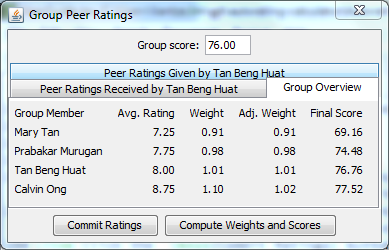
\includegraphics[width=\textwidth]{images/groupoverview}
%\caption{Autorated Weights and Scores of Group Members}
%\end{figure}
%
%\end{enumerate}
%
%\section{Opening Existing Assignment Score File}
%You may open an existing assignment score file (\texttt{*.xml}) to inspect scores, as well as to change settings and recalculate scores.
%\begin{enumerate}
%\item To open an existing score file, access the menu item \menu{File>Open\ldots} or press \keys{Ctrl+O}.
%\item Locate and select the \texttt{*.xml} file to open.
%\end{enumerate}
%
%\section{Exporting Data for Excel}
%The autorated scores can be exported for further processing in Excel.
%\begin{enumerate}
%\item Select \menu{File>Export\ldots} from the menu, or \keys{Ctrl+E}.
%\item Select a file name to save the exported data in. The file will be saved with a \texttt{.csv} extension. 
\includegraphics[height=1em]{csv}
%\item In Windows Explorer, locate the \texttt{.csv} file and double-click on it to open it in Excel.
%\item If warning messages are displayed, keep on clicking \keys{OK} or \keys{Yes} to ignore them.
%\item When the data is displayed, you may save the file as an \texttt{.xlsx} or \texttt{.xsl} Excel file, and continue processing it.
%
%\begin{figure}[H]
%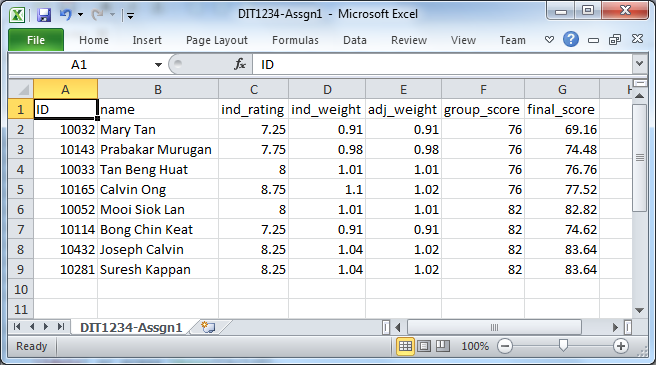
\includegraphics[width=\textwidth]{images/excel}
%\caption{Exported data in Excel}
%\end{figure}

%\end{enumerate}

\bibliographystyle{plain}
\bibliography{refs}
\end{document}